\documentclass[12pt,]{article}
\usepackage{lmodern}
\usepackage{amssymb,amsmath}
\usepackage{ifxetex,ifluatex}
\usepackage{fixltx2e} % provides \textsubscript
\ifnum 0\ifxetex 1\fi\ifluatex 1\fi=0 % if pdftex
  \usepackage[T1]{fontenc}
  \usepackage[utf8]{inputenc}
\else % if luatex or xelatex
  \ifxetex
    \usepackage{mathspec}
  \else
    \usepackage{fontspec}
  \fi
  \defaultfontfeatures{Ligatures=TeX,Scale=MatchLowercase}
\fi
% use upquote if available, for straight quotes in verbatim environments
\IfFileExists{upquote.sty}{\usepackage{upquote}}{}
% use microtype if available
\IfFileExists{microtype.sty}{%
\usepackage{microtype}
\UseMicrotypeSet[protrusion]{basicmath} % disable protrusion for tt fonts
}{}
\usepackage[margin=1in]{geometry}
\usepackage{hyperref}
\hypersetup{unicode=true,
            pdfborder={0 0 0},
            breaklinks=true}
\urlstyle{same}  % don't use monospace font for urls
\usepackage{graphicx,grffile}
\makeatletter
\def\maxwidth{\ifdim\Gin@nat@width>\linewidth\linewidth\else\Gin@nat@width\fi}
\def\maxheight{\ifdim\Gin@nat@height>\textheight\textheight\else\Gin@nat@height\fi}
\makeatother
% Scale images if necessary, so that they will not overflow the page
% margins by default, and it is still possible to overwrite the defaults
% using explicit options in \includegraphics[width, height, ...]{}
\setkeys{Gin}{width=\maxwidth,height=\maxheight,keepaspectratio}
\IfFileExists{parskip.sty}{%
\usepackage{parskip}
}{% else
\setlength{\parindent}{0pt}
\setlength{\parskip}{6pt plus 2pt minus 1pt}
}
\setlength{\emergencystretch}{3em}  % prevent overfull lines
\providecommand{\tightlist}{%
  \setlength{\itemsep}{0pt}\setlength{\parskip}{0pt}}
\setcounter{secnumdepth}{0}
% Redefines (sub)paragraphs to behave more like sections
\ifx\paragraph\undefined\else
\let\oldparagraph\paragraph
\renewcommand{\paragraph}[1]{\oldparagraph{#1}\mbox{}}
\fi
\ifx\subparagraph\undefined\else
\let\oldsubparagraph\subparagraph
\renewcommand{\subparagraph}[1]{\oldsubparagraph{#1}\mbox{}}
\fi

%%% Use protect on footnotes to avoid problems with footnotes in titles
\let\rmarkdownfootnote\footnote%
\def\footnote{\protect\rmarkdownfootnote}

%%% Change title format to be more compact
\usepackage{titling}

% Create subtitle command for use in maketitle
\newcommand{\subtitle}[1]{
  \posttitle{
    \begin{center}\large#1\end{center}
    }
}

\setlength{\droptitle}{-2em}

  \title{}
    \pretitle{\vspace{\droptitle}}
  \posttitle{}
    \author{}
    \preauthor{}\postauthor{}
    \date{}
    \predate{}\postdate{}
  
\usepackage{pdflscape}
\newcommand{\blandscape}{\begin{landscape}}
\newcommand{\elandscape}{\end{landscape}}

\begin{document}

\hypertarget{title}{%
\subsection{TITLE}\label{title}}

\emph{Authors}

\hypertarget{supplementary-methods}{%
\paragraph{Supplementary Methods}\label{supplementary-methods}}

~

\begin{center}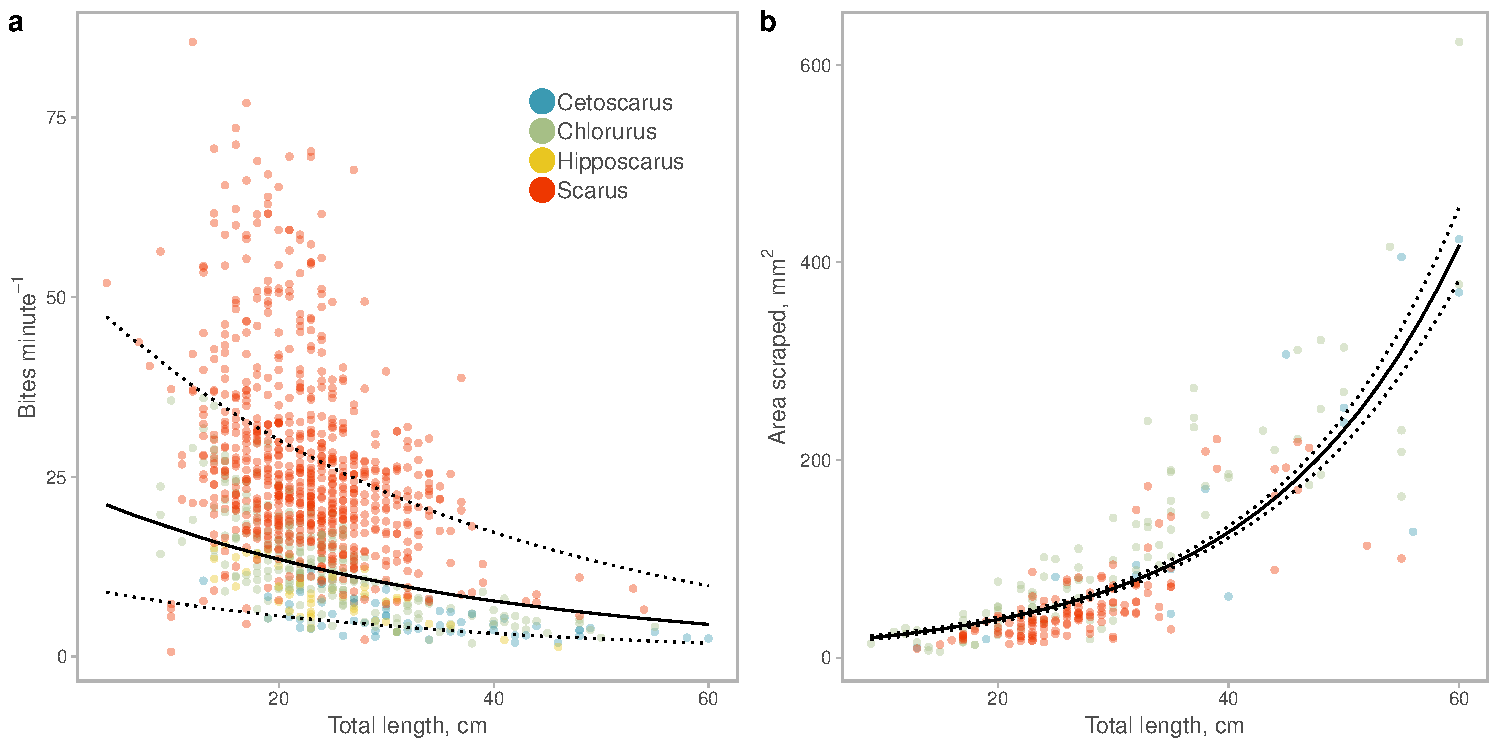
\includegraphics[width=480px]{../../figures/FigureS1_scrape_size} \end{center}

\textbf{Figure S1 \textbar{} Size effects on scraper bite rates (A) and
bite area (B).} Lines indicate median posterior predictions with 95\%
certainty intervals, excluding species and genera effects, across the
range of observed body sizes (total length, cm). Points are observed
bite rates or bite areas coloured by genera.

\newpage

\begin{center}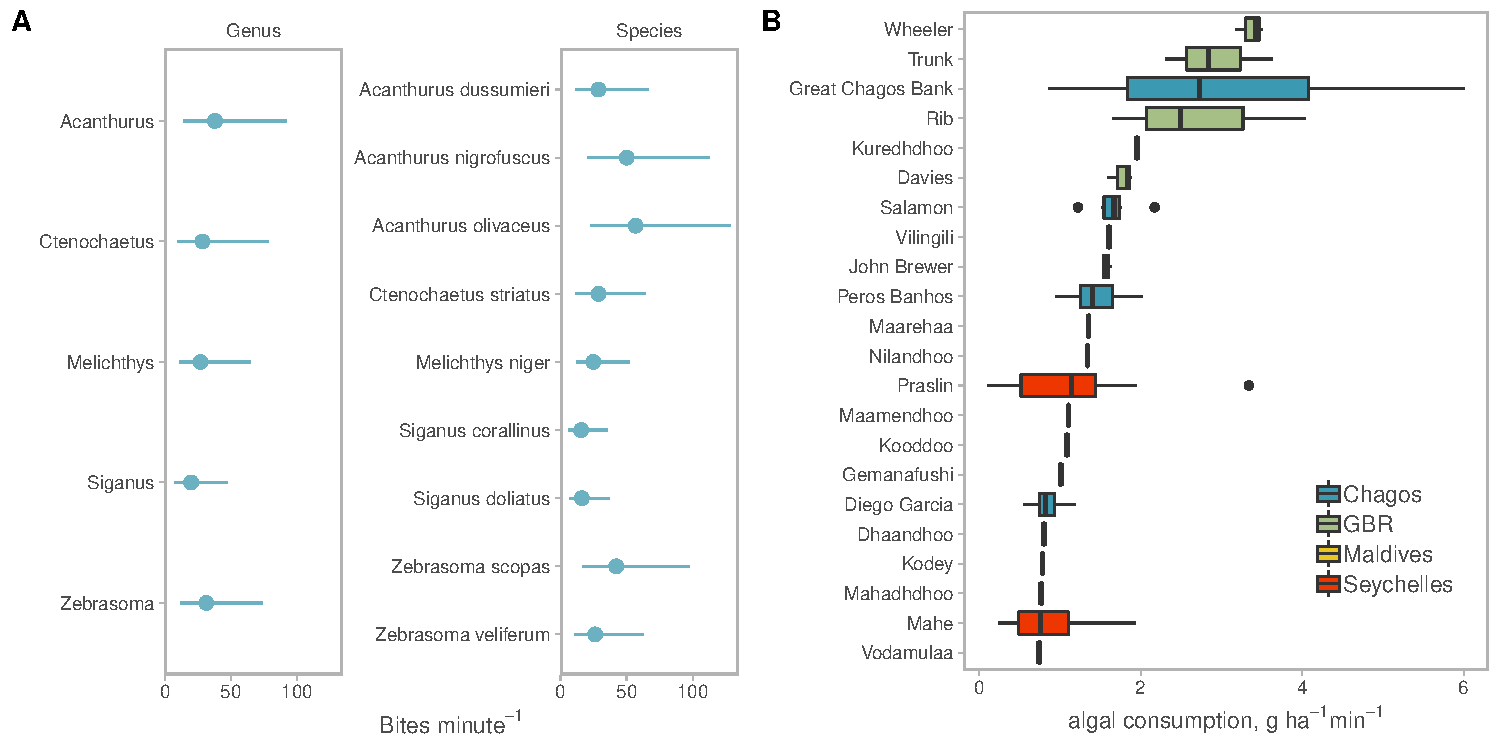
\includegraphics[width=480px]{../../figures/FigureS2_cropper_bites} \end{center}

\textbf{Figure S2 \textbar{} Cropper bite rate predictions (A) and
observed cropper function in UVC (B)} Predicted bite rates are median
posterior predictions with 95\% certainty intervals (A), and boxplots
are site-level observed cropping function for each reef, coloured by UVC
region.

\newpage

\begin{center}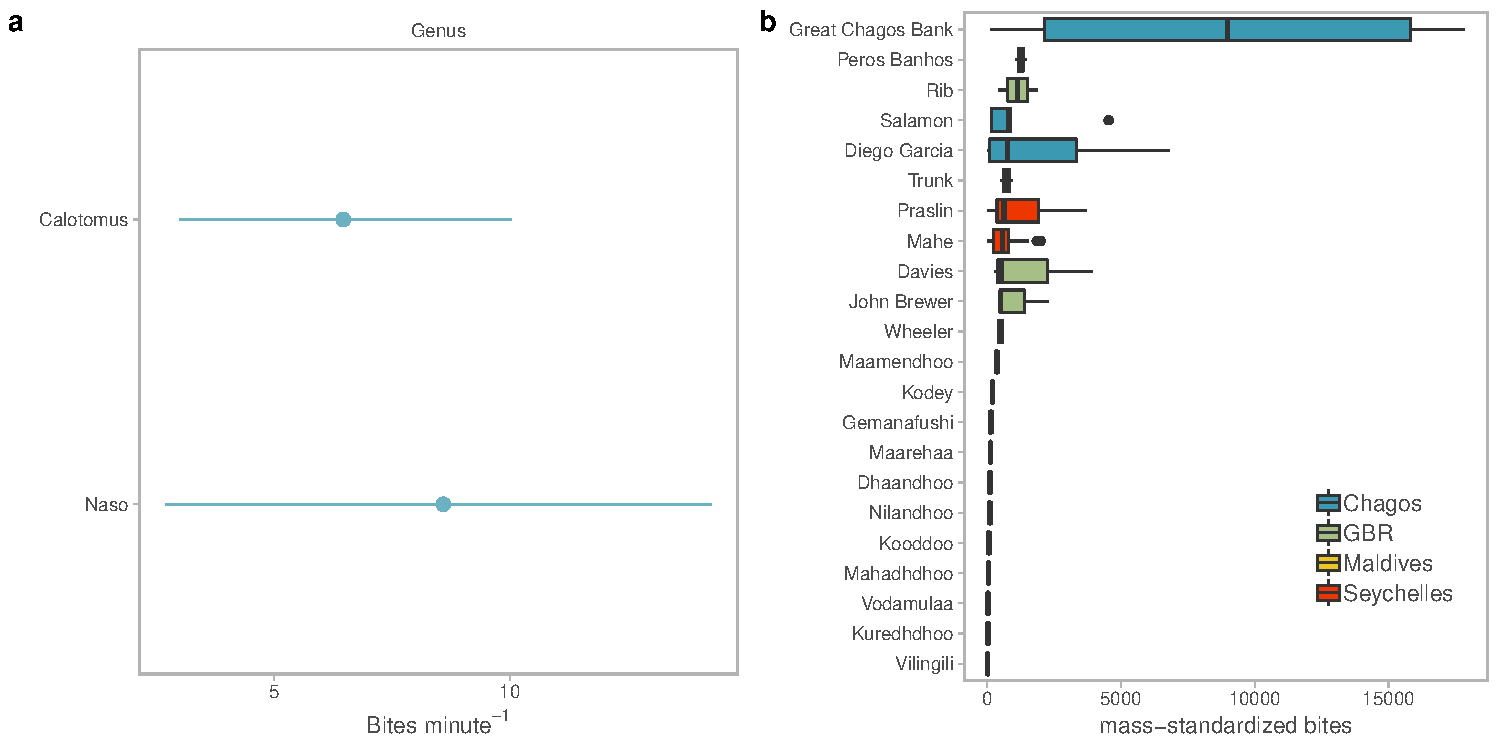
\includegraphics[width=480px]{../../figures/FigureS3_browser_bites} \end{center}

\textbf{Figure S3 \textbar{} Browser bite rate predictions (A) and
observed browser function in UVC (B)} Predicted bite rates are median
posterior predictions with 95\% certainty intervals (A), and boxplots
are site-level observed browsing function for each reef, coloured by UVC
region.

\newpage

\begin{center}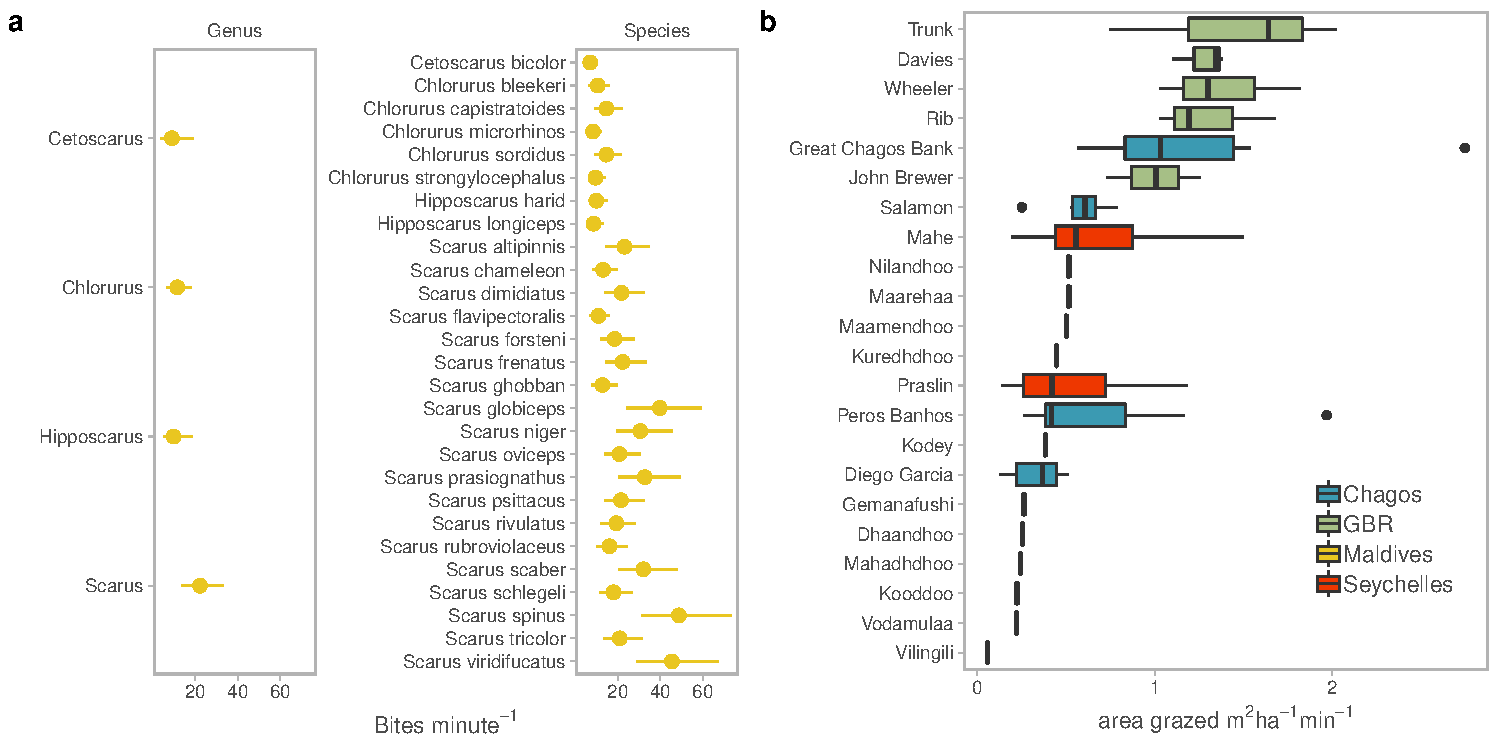
\includegraphics[width=480px]{../../figures/FigureS4_scraper_bites} \end{center}

\textbf{Figure S4 \textbar{} Scraper bite rate predictions (A) and
observed scraping function in UVC (B)} Predicted bite rates are median
posterior predictions with 95\% certainty intervals (A), and boxplots
are site-level observed scraping function for each reef, coloured by UVC
region.

\newpage

\begin{center}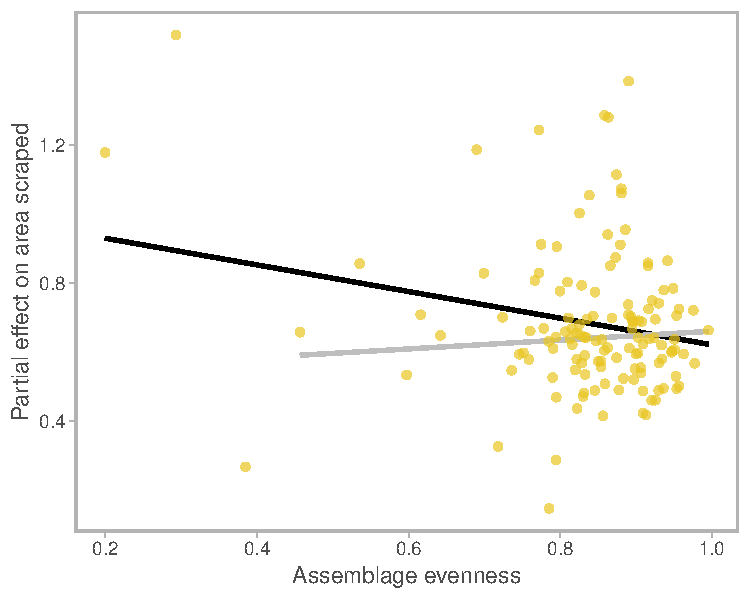
\includegraphics[width=480px]{../../figures/FigureS5_evenness} \end{center}

\textbf{Figure S5 \textbar{} Evenness effect on scraping function.}
Points are partial residuals from linear mixed effects model for
predicted evenness effect while excluding effects from other explanatory
covariates (e.g.~biomass, size, richness). Black line is fitted to full
dataset and grey line is fitted to evenness values \textgreater{} 0.4,
with 95\% bootstrapped confidence intervals.

\newpage


\end{document}
